
%(BEGIN_QUESTION)
% Copyright 2015, Tony R. Kuphaldt, released under the Creative Commons Attribution License (v 1.0)
% This means you may do almost anything with this work of mine, so long as you give me proper credit

\noindent

\vskip 5pt
\begin{center}
\vskip 5pt 
\textbf{Styresystemer -- Nivå 1 }
\vskip 5pt 
\textbf{Arbidsoppdrag på Stasjon 1}
\vskip 5pt 

\vskip 5pt 
\textbf{Programmering av gandsfjoden Gondol med Wago PFC 100}
\end{center}
\vskip 5pt 
\textbf{Introdusjon}

\vskip 5pt 
I Arbeidsoppdraget til gandsfjoden Gondol har du programmert stasjonen med Gand PLS 01. Nå skal du programmere stajonen med en Wago PLS 100. Stasjonen er ferdig oppkoblet og klar tl bruk.


\vskip 5pt 
\vskip 5pt 
%$$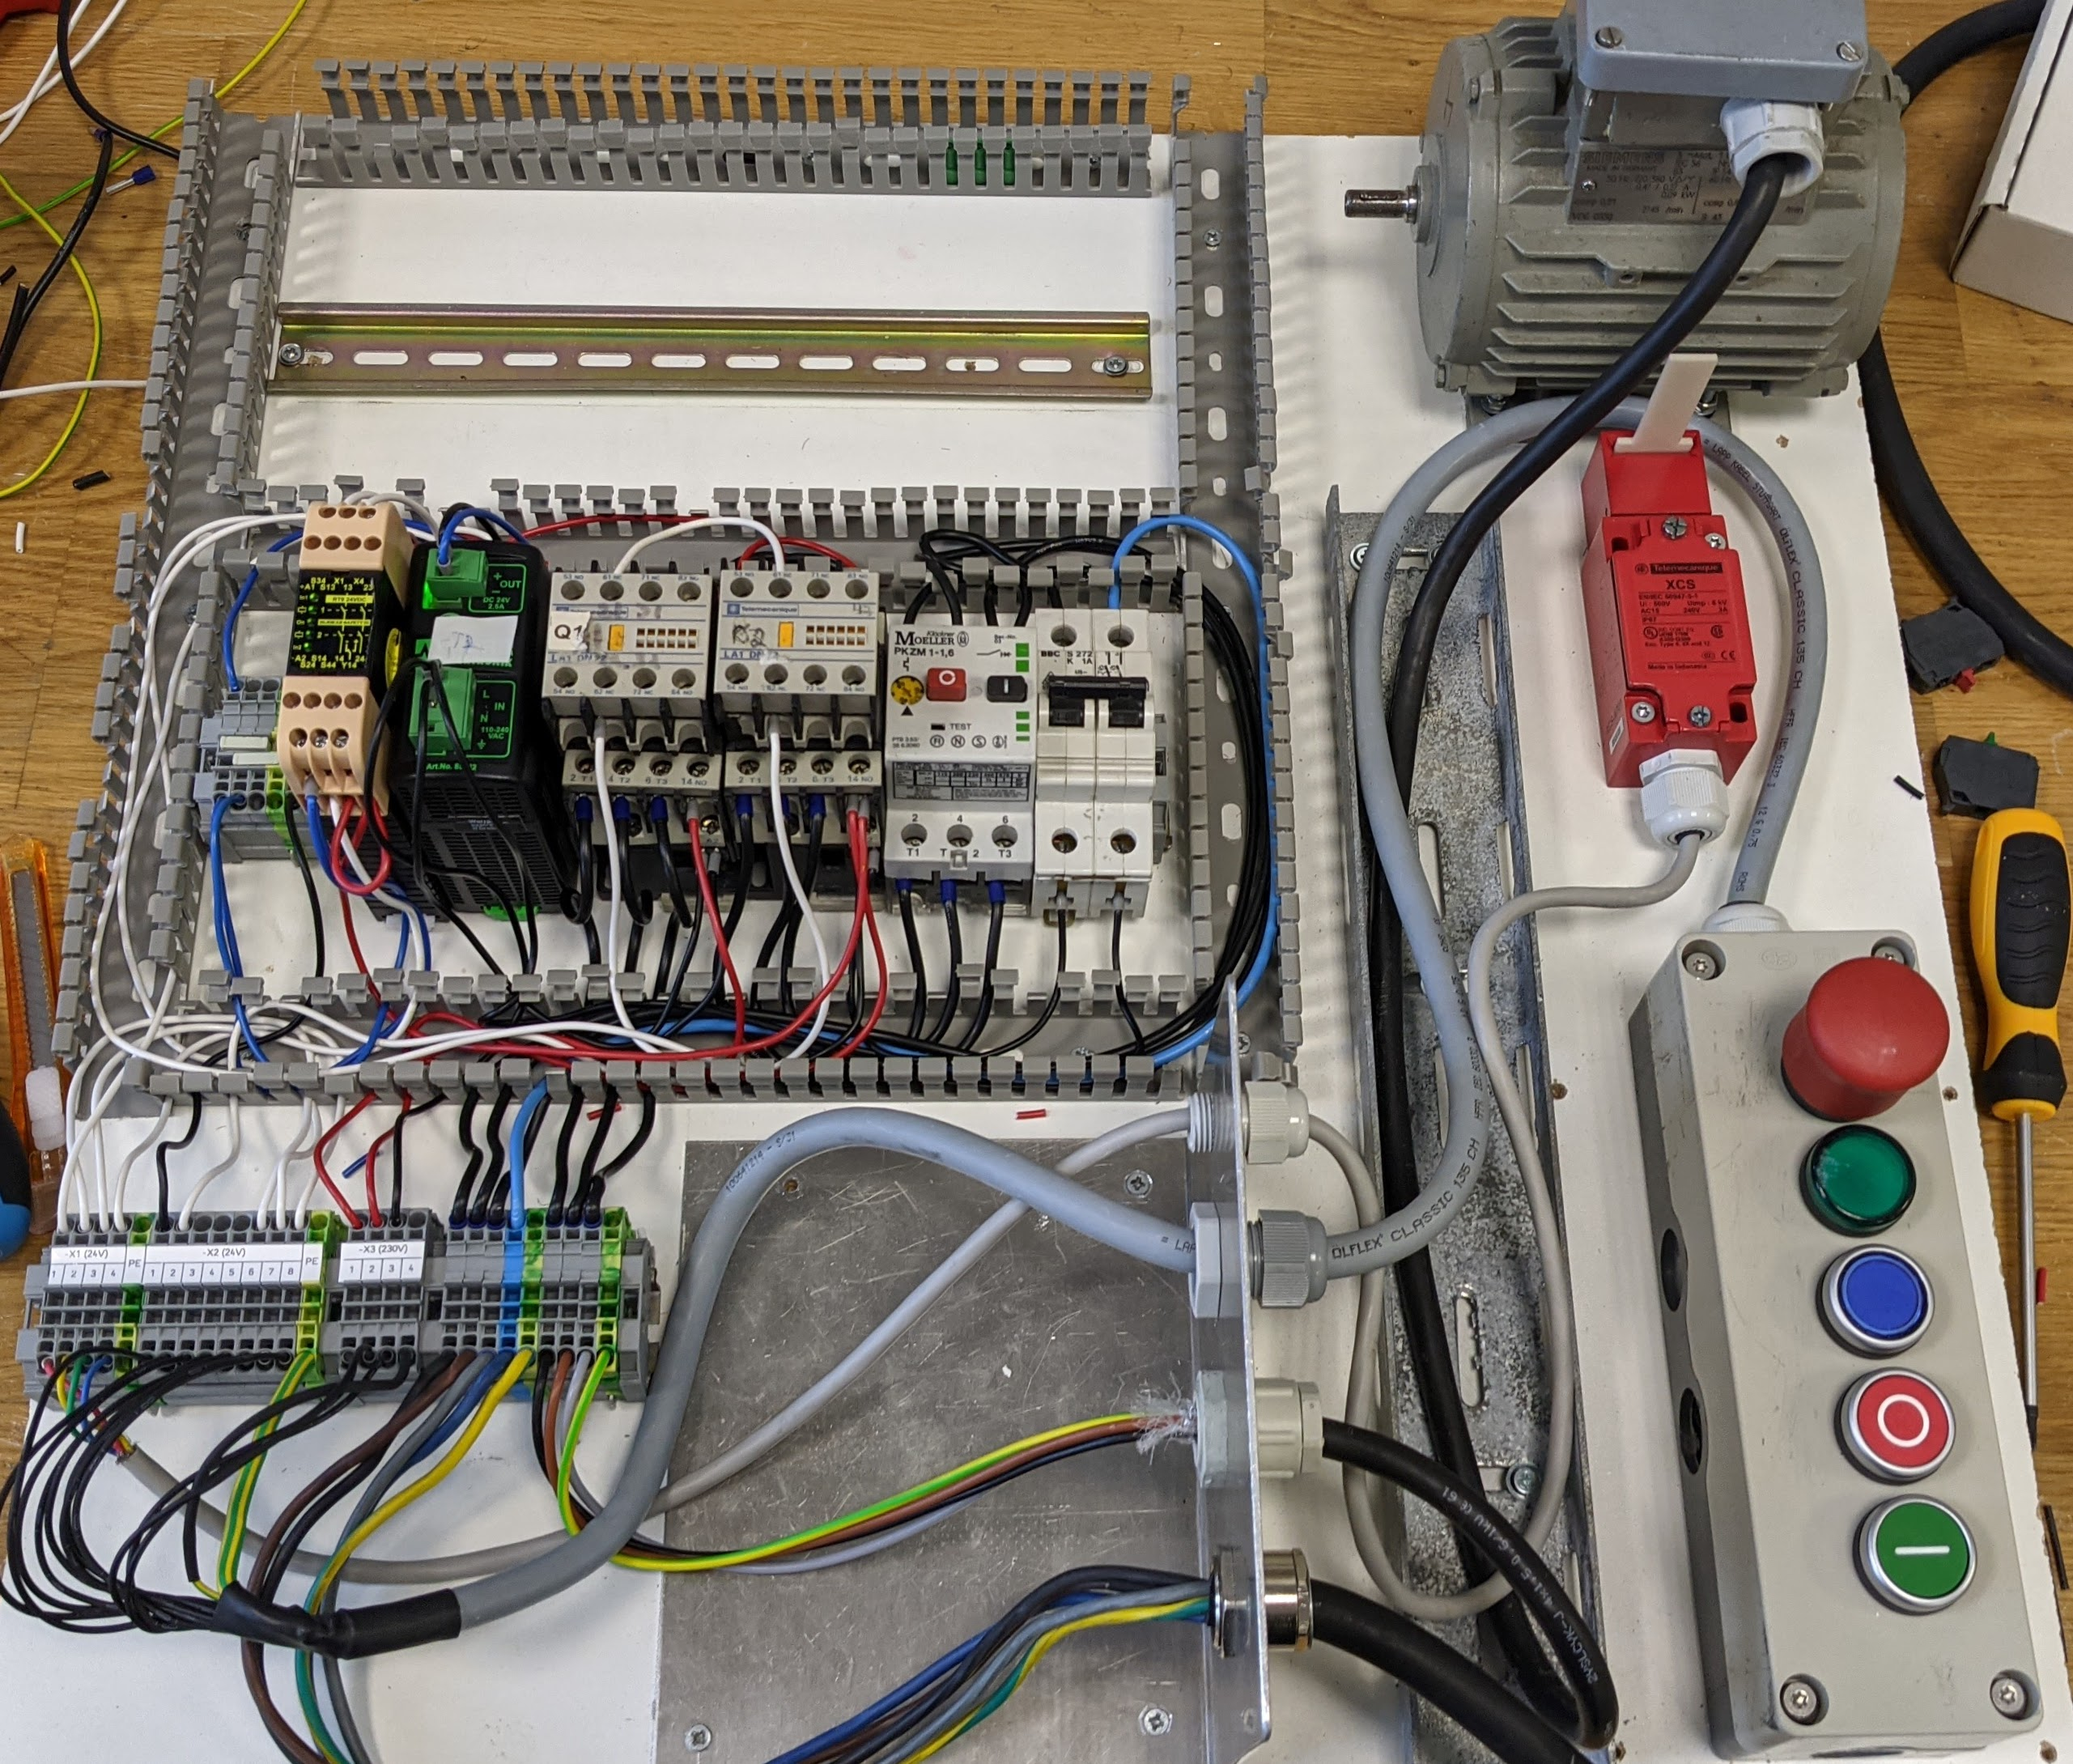
\includegraphics[width=13cm]{i04821x01.jpg}$$\\
\textbf{Teorioppgaver}
\vskip 5pt 
Nettsiden open PLC har gitt ut en stadard for hvordan en skal gå frem når en programmerer en PLS. I dette arbidsoppdraget skal du følge denne standarden den finner du her \href{https://rfka-my.sharepoint.com/:p:/g/personal/fred-olav_mosdal_skole_rogfk_no/EVXQGPn90WdIpSuDzhhkKIMBdVsQ1ozwb4glbCEAFAfRxg?e=Z9zaSK}{Presentasjon av prossedyren for programmering}. 

\vskip 10pt 
\textbf{Planlegging}

\begin{center}
\begin{tabular}{ | m{12cm} | m{1cm}| m{1cm} | } 
\hline
\multicolumn{3}{|c|}{\textbf{Sjekkliste for planlegging}} \\
\hline
Oppgave	& Elev & Lærer \\ 
\hline
	Eleven har definert IO signaler (IO-liste)&&\\
\hline
	Eleven har definert signaler til sentralt kontrollsystem &&\\
\hline
	
	Eleven har definert alle HMI signaler, overstyringer og overvåkningsdata &&\\
\hline
	Elevn har del programmet opp i logiske deler (min 2. ) &&\\ 	
	Styreprogramm og utgangsprogramm &&\\
	\hline
	Eleven har laget POU for hver av de logiske delene &&\\
	og programmene er godt kommentert &&\\
	\hline
	Eleven har koble de fysike IO-ene mot variabler i programmet &&\\
	\hline
\end{tabular}
\end{center}
\vskip 10pt 
\vskip 10pt 
\textbf{Gjennomføring}


\vskip 10pt 
\textbf{Dokumentasjon}


Beskriv hvordan du planlegger, gjennomfører og dokumenterer denne jobben. 












\underbar{file i04822}
\vfil \eject
%(END_QUESTION)





%(BEGIN_ANSWER)


%(END_ANSWER)





%(BEGIN_NOTES)


%INDEX% Arbeisdoppdrag, Styresystemer, Nivå 1, Stasjon01, Programmering av Gandsfjorden Gondol med Wago  PFC100

%(END_NOTES)


